\chapter{Dipole radiation}
Radiation means the generation of electromagnetic waves, which then propagate away from the source to infinity. Classically, electromagnetic waves are created by charged particles accelerating, or, equivalently, currents varying in time. There is no radiation in case of electric and magnetic fields of a point charge moving with constant velocity. The energy in the electromagnetic field is transported along with the particle, but does not propagate away toward infinity. But if the charge velocity is not constant there must be radiation.\\
As we start the study of radiation, it is interesting to remember that the classical field theory was developed from experiments and observations on macroscopic objects such as charged bodies, insulators, conductors, current-carrying wires, and magnets. The classical theory is therefore at its best when applied to macroscopic electromagnetic phenomena. So, for example, the theory applies to radiation of radio waves by an antenna, or microwaves by a cavity resonator. In this book we concentrate mainly on systems of that kind.\\
 However, much of the radiation around us-in fact much of the radiation in the Universe-comes from microscopic systems and must be described by quantum electrodynamics. For example, sunlight, light from the filament of an incandescent bulb, fluorescent light, or laser light can only be explained by quantum considerations of individual atoms, molecules, or systems of atoms. For these systems the classical theory does not really apply, except perhaps in a qualitative, heuristic way. Only quantum electrodynamics can properly describe radiation by an atom. Despite its limited applicability, the classical theory of radiation is an important part of electromagnetism. Quantum electrodynamics, which has limitations of its own, relies on a foundation of classical electrodynamics.\\
 \newpage
 \section{Electric dipole radiation}
 Picture two tiny metal spheres separated by a distance $d$ and connected by a fine wire (figure below); at time $t$ the charge on the upper sphere is $q(t)$, and the charge on the lower sphere is $-q(t)$. Suppose that we drive the charge back and forth through the wire, from one end to the other, at an angular frequency $\omega$ :
 $$
 q(t)=q_{0} \cos (\omega t)
 $$
 \begin{figure}[H]
 	\centering
 	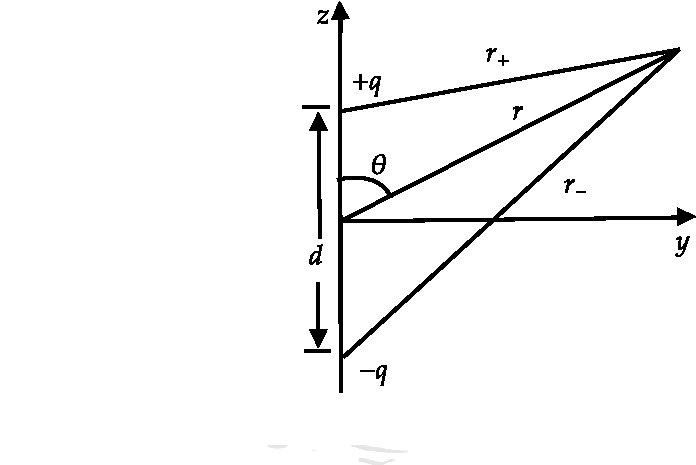
\includegraphics[height=5cm,width=8cm]{dipole-crop}
 	\caption{}
 	\label{}
 \end{figure}
 The result is an oscillating electric dipole:
 $$
 \mathbf{p}(t)=p_{0} \cos (\omega t) \hat{\mathbf{z}}
 $$
 where
 $$
 p_{0}=q_{0} d
 $$
 is the maximum value of the dipole moment.
 With the approximation of
 $$
 d \ll \frac{\lambda}{2 \pi} \ll r
 $$
 you should not forget that $\frac{\lambda}{2 \pi}=\frac{c}{\omega}$ we can calculate the potentials\\
 $$
 V(r, \theta, t)=-\frac{p_{0} \omega}{4 \pi \epsilon_{0} c}\left(\frac{\cos \theta}{r}\right) \sin [\omega(t-r / c)]
 $$
 and
 $$
 \mathbf{A}(r, \theta, t)=-\frac{\mu_{0} p_{0} \omega}{4 \pi r} \sin [\omega(t-r / c)] \hat{\mathbf{z}}
 $$
 Hence we get the fields
 $$
 \mathbf{E}=-\nabla V-\frac{\partial \mathbf{A}}{\partial t}=-\frac{\mu_{0} p_{0} \omega^{2}}{4 \pi}\left(\frac{\sin \theta}{r}\right) \cos [\omega(t-r / c)] \hat{\boldsymbol{\theta}}
 $$
 and
 $$
 \mathbf{B}=\nabla \times \mathbf{A}=-\frac{\mu_{0} p_{0} \omega^{2}}{4 \pi c}\left(\frac{\sin \theta}{r}\right) \cos [\omega(t-r / c)] \hat{\phi}
 $$
 The energy radiated by an oscillating electric dipole is determined by the Poynting vector:
 $$\mathbf{S}(\mathbf{r}, t)=\frac{1}{\mu_{0}}(\mathbf{E} \times \mathbf{B})=\frac{\mu_{0}}{c}\left\{\frac{p_{0} \omega^{2}}{4 \pi}\left(\frac{\sin \theta}{r}\right) \cos [\omega(t-r / c)]\right\}^{2} \hat{\mathbf{r}}$$
 The intensity is obtained by averaging (in time) over a complete cycle:
 $$\langle\mathbf{S}\rangle=\left(\frac{\mu_{0} p_{0}^{2} \omega^{4}}{32 \pi^{2} c}\right) \frac{\sin ^{2} \theta}{r^{2}} \hat{\mathbf{r}}$$
 The total power radiated is found by integrating $\langle\mathbf{S}\rangle$ over a sphere of radius $r$ :
 $$ \langle P\rangle=\int\langle\mathbf{S}\rangle \cdot d \mathbf{a}=\frac{\mu_{0} p_{0}^{2} \omega^{4}}{32 \pi^{2} c} \int \frac{\sin ^{2} \theta}{r^{2}} r^{2} \sin \theta d \theta d \phi=\frac{\mu_{0} p_{0}^{2} \omega^{4}}{12 \pi c}$$
 \section{Magnetic dipole radiations}
 Suppose now that we have a wire loop of radius $b$ (figure below) around which we drive an alternating current:
 $$I(t)=I_{0} \cos (\omega t)$$
 This is a model for an oscillating magnetic dipole,
 $$
 \mathbf{m}(t)=\pi b^{2} I(t) \hat{\mathbf{z}}=m_{0} \cos (\omega t) \hat{\mathbf{z}}
 $$
 \begin{figure}[H]
 	\centering
 	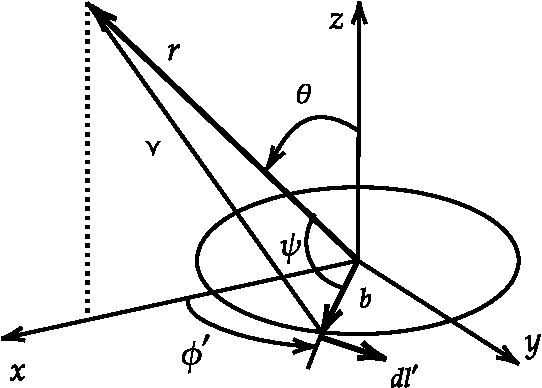
\includegraphics[height=4.5cm,width=7cm]{m dipole-crop}
 	\caption{}
 	\label{}
 \end{figure}
 where the maximum value of the magnetic dipole moment is.\\
 $$m_{0}=\pi b^{2} I_{0}$$
 Again with the assumption of
 $$
 b \ll \frac{\lambda}{2 \pi} \ll r
 $$
 we get the potentials and fields \\
 $$\mathbf{A}(r, \theta, t)=-\frac{\mu_{0} m_{0} \omega}{4 \pi c}\left(\frac{\sin \theta}{r}\right) \sin [\omega(t-r / c)] \hat{\phi}$$
 There is no electric scalar potential as there is no static charge. Hence the fields\\
 $$\mathbf{E}=-\frac{\partial \mathbf{A}}{\partial t}=\frac{\mu_{0} m_{0} \omega^{2}}{4 \pi c}\left(\frac{\sin \theta}{r}\right) \cos [\omega(t-r / c)] \hat{\phi}$$
 and
 $$\mathbf{B}=\nabla \times \mathbf{A}=-\frac{\mu_{0} m_{0} \omega^{2}}{4 \pi c^{2}}\left(\frac{\sin \theta}{r}\right) \cos [\omega(t-r / c)] \hat{\boldsymbol{\theta}}$$
 The Poynting vector 
 $$\mathbf{S}(\mathbf{r}, t)=\frac{1}{\mu_{0}}(\mathbf{E} \times \mathbf{B})=\frac{\mu_{0}}{c}\left\{\frac{m_{0} \omega^{2}}{4 \pi c}\left(\frac{\sin \theta}{r}\right) \cos [\omega(t-r / c)]\right\}^{2} \hat{\mathbf{r}}$$
 time average of Poynting vector
 $$
 \langle\mathbf{S}\rangle=\left(\frac{\mu_{0} m_{0}^{2} \omega^{4}}{32 \pi^{2} c^{3}}\right) \frac{\sin ^{2} \theta}{r^{2}} \hat{\mathbf{r}}
 $$
 the total radiated power
 $$
 \langle P\rangle=\frac{\mu_{0} m_{0}^{2} \omega^{4}}{12 \pi c^{3}}
 $$
 \begin{note}
 	If you compare the formula for power for electric and magnetic dipole radiation you get
 	$$\frac{P_{\text {magnetic }}}{P_{\text {electric }}}=\left(\frac{m_{0}}{p_{0} c}\right)^{2}$$
 \end{note}
 
\section{Radiation from a arbitrary source}
Power radiated from arbitrary electric source whose electric dipole moment is changing with respect to time\\
$$P_{\operatorname{rad}}\left(t_{0}\right) \cong \frac{\mu_{0}}{6 \pi c}\left[\ddot{p}\left(t_{0}\right)\right]^{2}$$
Power radiated from arbitrary magnetic source whose magnetic dipole moment is changing with respect to time
$$P_{\mathrm{rad}}\left(t_{0}\right) \cong \frac{\mu_{0}}{6 \pi c^{3}}\left[\ddot{m}\left(t_{0}\right)\right]^{2}$$
\begin{exercise}
 A particle moving straight line with velocity $v=v_{0}+\alpha t$. How much energy does it radiate?
\end{exercise}
\begin{answer}
The position of the particle
$$
x=x_{0}+v_{0} t+\frac{1}{2} \alpha t^{2}
$$
Now dipole moment
$$
\mathbf{p}=q x \hat{i}
$$
$$\begin{aligned}
	&\Rightarrow p=q\left(x_{0}+v_{0} t+\frac{1}{2} \alpha t^{2}\right) \\
	&\Rightarrow \ddot{p}=q \alpha \\
	&\text { Power }=\frac{\mu_{0}}{6 \pi c} q^{2} \alpha^{2}
\end{aligned}$$
This is the famous larmor formula.\\
This formula can be used for a point charge moving with acceleration $\alpha$	
\end{answer}
\begin{exercise}
	 A parallel-plate capacitor $C$, with plate separation $d$, is given an initial charge $(\pm) Q_{0}$. It is then connected to a resistor $R$, and discharges, $Q(t)=Q_{0} e^{-t / R C}$. What fraction of its initial energy $\left(Q_{0}^{2} / 2 C\right)$ does it radiate away?
\end{exercise}
\begin{answer}
	Power radiated is
	$$
	\frac{\mu_{0}}{6 \pi c} \ddot{p}^{2}
	$$
	In our case
	$$
	p=Q d, \text { so } \ddot{p}=\ddot{Q} d=Q_{0}\left(\frac{1}{R C}\right)^{2} e^{-t / R C} d
	$$
	So power radiated
	$$
	\frac{d W_{r}}{d t}=\frac{\mu_{0}}{6 \pi c} \frac{\left(Q_{0} d\right)^{2}}{(R C)^{4}} e^{-2 t / R C}
	$$
	The total energy radiated is
	$$
	\begin{aligned}
	W_{r} &=\frac{\mu_{0}}{6 \pi c} \frac{\left(Q_{0} d\right)^{2}}{(R C)^{4}} \int_{0}^{\infty} e^{-2 t / R C} d t \\
	&=\left.\frac{\mu_{0}}{6 \pi c} \frac{\left(Q_{0} d\right)^{2}}{(R C)^{4}}\left[-\frac{R C}{2} e^{-2 t / R C}\right]\right|_{0} ^{\infty} \\
	&=\frac{\mu_{0}}{6 \pi c} \frac{\left(Q_{0} d\right)^{2}}{(R C)^{4}} \frac{R C}{2}=\frac{\mu_{0}}{12 \pi c} \frac{\left(Q_{0} d\right)^{2}}{(R C)^{3}}
	\end{aligned}
	$$
\end{answer}
\begin{exercise}
 An electron is released from rest and falls under the influence of gravity. In the first centimeter, what fraction of the potential energy lost is radiated away?
\end{exercise}
\begin{answer}
Let the $y$ direction is in the downwards direction then\\
$\mathbf{p}=-e y \hat{\mathbf{y}}, y=\frac{1}{2} g t^{2}, \text { so } \mathbf{p}=-\frac{1}{2} g e t^{2} \hat{\mathbf{y}} ; \ddot{\mathbf{p}}=-g e \hat{\mathbf{y}}$\\
Hence the power radiated is
$$
P=\frac{\mu_{0}}{6 \pi c}(g e)^{2}
$$
Now the time the charge takes to fall a distance $h$ is given by $h=\frac{1}{2} g t^{2} \Rightarrow t=\sqrt{2 h / g}$, so the energy radiated in falling a distance $h$ is
$$
U_{\mathrm{rad}}=P t=\frac{\mu_{0}(g e)^{2}}{6 \pi c} \sqrt{2 h / g}
$$
The potential energy lost is $U_{\text {pot }}=m g h$. So the fraction is
$$
\begin{aligned}
f &=\frac{U_{\mathrm{rad}}}{U_{\mathrm{pot}}}=\frac{\mu_{0} g^{2} e^{2}}{6 \pi c} \sqrt{\frac{2 h}{g} \frac{1}{m g h}}=\frac{\mu_{0} e^{2}}{6 \pi m c} \sqrt{\frac{2 g}{h}} \\
&=\frac{\left(4 \pi \times 10^{-7}\right)\left(1.6 \times 10^{-19}\right)^{2}}{6 \pi\left(9.11 \times 10^{-31}\right)\left(3 \times 10^{8}\right)} \sqrt{\frac{(2)(9.8)}{(0.01)}}=2.76 \times 10^{-22}
\end{aligned}
$$
\end{answer}
\begin{exercise}
	 In Bohr's theory of hydrogen, the electron in its ground state was supposed to travel in a circle of radius $5 \times 10^{-11} \mathrm{~m}$, held in orbit by the Coulomb attraction of the proton. According to classical electrodynamics, this electron should radiate, and hence spiral in to the nucleus. Show that $v \ll c$ for most of the trip (so you can use the Larmor formula), and calculate the lifespan of Bohr's atom. (Assume each revolution is essentially circular.)
\end{exercise}
\begin{answer}
$$
F=\frac{1}{4 \pi \epsilon_{0}} \frac{q^{2}}{r^{2}}=m a=m \frac{v^{2}}{r} \Rightarrow v=\sqrt{\frac{1}{4 \pi \epsilon_{0}} \frac{q^{2}}{m r}}
$$
At the beginning $\left(r_{0}=0.5 \mathrm{~A}\right)$
$$
\begin{aligned}
\frac{v}{c} &=\left[\frac{\left(1.6 \times 10^{-19}\right)^{2}}{4 \pi\left(8.85 \times 10^{-12}\right)\left(9.11 \times 10^{-31}\right)\left(5 \times 10^{-11}\right)}\right]^{-\frac{1}{2}} \frac{1}{3 \times 10^{8}} \\
&=0.0075
\end{aligned}
$$
and when the radius is one hundredth of this $v / c$ is only 10 times greater $(0.075)$, so for most of the trip the velocity is safely nonrelativistic. From the Larmor formula,
$$P=\frac{\mu_{0} q^{2}}{6 \pi c}\left(\frac{v^{2}}{r}\right)^{2}=\frac{\mu_{0} q^{2}}{6 \pi \epsilon_{0}}\left(\frac{1}{4 \pi \epsilon_{0}} \frac{q^{2}}{m r^{2}}\right)^{2}$$
since $a=v^{2} / r$, and $P=-d U / d t$ where $U$ is the (total) energy of the electron
$$
\begin{aligned}
	U &=U_{\mathrm{kin}}+U_{\mathrm{pot}}=\frac{1}{2} m v^{2}-\frac{1}{4 \pi \epsilon_{0}} \frac{q^{2}}{r} \\
	&=\frac{1}{2}\left(\frac{1}{4 \pi \epsilon_{0}} \frac{q^{2}}{r}\right)-\frac{1}{4 \pi \epsilon_{0}} \frac{q^{2}}{r} \\
	&=-\frac{1}{8 \pi \epsilon_{0}} \frac{q^{2}}{r}
\end{aligned}$$
So
$$
-\frac{d U}{d t}=-\frac{1}{8 \pi \epsilon_{0}} \frac{q^{2}}{r^{2}} \frac{d r}{d t}=P=\frac{q^{2}}{6 \pi \epsilon_{0} c^{3}}\left(\frac{1}{4 \pi \epsilon_{0}} \frac{q^{2}}{m r^{2}}\right)^{2}
$$
and hence
$$
\frac{d r}{d t}=-\frac{1}{3 c}\left(\frac{q^{2}}{2 \pi \epsilon_{0} m c}\right)^{2} \frac{1}{r^{2}}
$$
or
$$
\begin{aligned}
d t &=-3 c\left(\frac{2 \pi \epsilon_{0} m c}{q^{2}}\right)^{2} r^{2} d r \Rightarrow t \\
&=-3 c\left(\frac{2 \pi \epsilon_{0} m c}{q^{2}}\right)^{2} \int_{r_{0}}^{0} r^{2} d r \\
&=c\left(\frac{2 \pi \epsilon_{0} m c}{q^{2}}\right)^{2} r_{0}^{3}
\end{aligned}
$$
or
$$
\begin{aligned}
t=&\left(3 \times 10^{8}\right) \times \\
&\left[\frac{2 \pi\left(8.85 \times 10^{-12}\right)\left(9.11 \times 10^{-31}\right)\left(3 \times 10^{8}\right)}{\left(1.6 \times 10^{-19}\right)^{2}}\right]^{2}\left(5 \times 10^{-11}\right)^{3} \\
=& 1.3 \times 10^{-11} \mathrm{~s}
\end{aligned}
$$	
\end{answer}

\section{Lagrangian and hamiltonian of a charged particle in a Electromagnetic field}
The force experienced by a particle of charge q at rest in an electric field of intensity E is given by
$$F_1=qE$$
The force experienced by a moving charge q in a magnetic field B is given by\\
$$F_2=q(v\times B)$$
Where V  is the velocity of the particle.The direction of $F_2$ is perpendicular to both v and B.\\
Total force on a uniformly moving charged particle of charge q is the sum of $F_1$ and $F_2$\\
$$F=F_1+F_2=qE+q(v\times B)$$
The above equation is known as lorentz formula.\\
Maxwell's equation in empty space is given by\\
$\nabla \cdot E=\frac{\rho}{\epsilon_0}$\\
$\nabla \cdot B=0$\\
$\nabla \times E=-\frac{\partial B}{\partial t}$\\
$\nabla \times B=\mu_0(J+\epsilon_0\frac{\partial E}{\partial t})$\\
We know that if $\nabla \cdot B=0$ ,B can be expressed as a curl of some vector A\\
$$B=\nabla \times A$$
Substitute this equation in $\nabla \times E=-\frac{\partial B}{\partial t}$\\
$\nabla \times E=-\frac{\partial B}{\partial t}=-\frac{\partial}{\partial t}(\nabla \times A)=-\nabla \times \frac{\partial A}{\partial t}$\\
$\therefore E=-\frac{\partial A}{\partial t}-\nabla s$ ,since curl of gradient is always zero and s is  scalar function\\
The lorentz force in terms of scalar potential s and vector potential A is given by\\
$$F=q\left[ E+v\times B\right] $$
$$F=q\left[ -\frac{\partial A}{\partial t}-\nabla s+(v\times \nabla \times A)\right] $$
Let us consider the last part $v\times(\nabla \times A)$\\
$$v\times(\nabla \times A)=\nabla (A\cdot v)-(\nabla \cdot v)A$$
Also $A=A(x,y,z,t)$\\
Therfore total time derivative of A is given by\\
$\frac{dA}{dt}=\frac{\partial A}{\partial x} \dot{x}+\frac{\partial A}{\partial y} \dot{y}+\frac{\partial A}{\partial z} \dot{z}+\frac{\partial A}{\partial t}=\frac{\partial A}{\partial x} v_x+\frac{\partial A}{\partial y} v_y+\frac{\partial A}{\partial z} v_z+\frac{\partial A}{\partial t}$\\
$=(\hat{i}v_x+\hat{j}v_y+\hat{k}v_z)\cdot \left( \hat{i}\frac{\partial A}{\partial x}+\hat{j}\frac{\partial A}{\partial y}+\hat{k}\frac{\partial A}{\partial z}\right) +\frac{\partial A}{\partial t}=v \cdot \nabla \mathbf{A}+\frac{\partial \mathbf{A}}{d t}$ \\
$$v \cdot\nabla \mathbf{A}=\frac{d \mathbf{A}}{d t}-\frac{\partial \mathbf{A}}{\partial t}$$
Substituting this value in 
$$v\times(\nabla \times A)=\nabla (A\cdot v)-(\nabla \cdot v)A$$
we will get \\
$$\mathrm{v} \times(\nabla \times \mathbf{A})=\nabla(\mathbf{A} \cdot \mathrm{v})-\frac{d \mathbf{A}}{d t}+\frac{\partial \mathbf{A}}{\partial t}$$
Then F becomes\\
$$F=q\left[ -\frac{\partial A}{\partial t}-\nabla s+(v\times \nabla \times A)\right] $$
$$\begin{aligned}
\mathbf{F} &=q\left[-\frac{\partial \mathbf{A}}{d t}-\nabla s+\left\{\nabla(\mathbf{A} \cdot \mathrm{v})-\frac{d \mathbf{A}}{d t}+\frac{\partial \mathbf{A}}{\partial t}\right\}\right] \\
&=q\left[-\nabla s+\left\{\nabla(\mathbf{A} \cdot \mathrm{v})-\frac{d \mathbf{A}}{d t}\right\}\right] \\
&=q\left[-\nabla(s-\mathbf{A} \cdot \mathrm{v})-\frac{d \mathbf{A}}{d t}\right]
\end{aligned}$$
The $x$-component of the force is given by
$$
\begin{aligned}
F_{x} &=q\left[\{-\nabla(s-\mathbf{A} \cdot \mathrm{v})\}_{x}-\frac{d \mathbf{A}_{x}}{d t}\right] \\
&=q\left[-\frac{\partial}{\partial x}(s-\mathbf{A} \cdot \mathrm{v})-\frac{d \mathbf{A}_{x}}{d t}\right] \\
\text { or } \quad F_{x} &=q\left[-\frac{\partial}{\partial x}(s-\mathbf{A} \cdot \mathrm{v})-\frac{d}{d t}\left\{\frac{\partial}{\partial \mathrm{v}_{x}}(\mathbf{A} \cdot \mathrm{v}\}\right]\right.
\end{aligned}
$$
$q s \text { is independent of velocity } \mathrm{v}_{x} \text { i.e. } \frac{\partial(q s)}{\partial \mathrm{v}_{x}}=0$
So we can add that term to the above equation, it will not make any change.\\
After rewritting\\
$$\begin{aligned}
&F_{x}=-\frac{\partial U}{\partial x}-\frac{d}{d t} \frac{\partial U}{\partial \mathrm{v}_{\mathrm{x}}} \\
&U=q s-q(\mathbf{A} \cdot \mathbf{v})
\end{aligned}$$
FRom these it is clear that  U is a function of x and v ie $q_k$ and $\dot{q_k}$
U is called generalized potential or velocity dependent potential.\\
\paragraph{Lagrangian }
$L=T-U=T-\{q s-q(\mathbf{A} \cdot \mathbf{v}) .\}=T-q s+q(\mathbf{A} \cdot \mathbf{v})$\\
T=kinetic energy.$T=\frac{1}{2}mv^2$
$$L=\frac{1}{2}mv^2-q s+q(\mathbf{A} \cdot \mathbf{v})$$
\textbf{Momentum} $P_K=\frac{\partial L}{\partial \dot{q_k}}=\frac{\partial L}{\partial v_k}=mv_k+qA=mv+qA$\\
\paragraph{Hamiltonian}
$$\begin{aligned}
H &=\sum_{k} p_{k} \dot{q}_{k}-L \\
&=\sum_{k} p_{k} \dot{r}_{k}-L \\
&=\sum_{k} p_{k} v_{k}-L \\
&=\sum_{k}\left(m v_{k}+q A_{k}\right) v_{k}-\left[\frac{1}{2} m v^{2}-q s+q(\mathbf{v} \cdot \mathbf{A})\right] \\
&=\sum_{k}\left(m v_{k}^{2}+q A_{k} v_{k}\right)-\frac{1}{2} m v^{2}+q s-q(\mathbf{v} \cdot \mathbf{A}) \\
&=m v^{2}+q(\mathbf{A} \cdot \mathbf{v})-\frac{1}{2} m v^{2}+q s-q(\mathbf{v} \cdot \mathbf{A}) \\
&=\frac{1}{2} m v^{2}+q s
\end{aligned}$$

\newpage
\begin{abox}
	Previous Year solutions
\end{abox}
\begin{enumerate}
	\begin{minipage}{\textwidth}
		\item An electron is decelerated at a constant rate starting from an initial velocity $u$ (where $u<<c$ ) to $u / 2$ during which it travels a distance $s$. The amount of energy lost to radiation is
		\exyear{NET 2017}
	\end{minipage}
	\begin{tasks}(2)
		\task[\textbf{A.}] $\frac{\mu_{0} e^{2} u^{2}}{3 \pi m c^{2} s}$
		\task[\textbf{B.}]$\frac{\mu_{0} e^{2} u^{2}}{6 \pi m c^{2} s}$
		\task[\textbf{C.}]$\frac{\mu_{0} e^{2} u}{8 \pi m c s}$
		\task[\textbf{D.}]$\frac{\mu_{0} e^{2} u}{16 \pi m c s}$
	\end{tasks}
	\begin{answer}
		$\text { Total power radiated } P=\frac{\mu_{0} q^{2} a^{2}}{6 \pi c}$\\
		$\text { Total energy radiated in time } t \text { is } E=P \cdot t=\frac{\mu_{0} e^{2} a^{2}}{6 \pi c} \cdot t=\frac{\mu_{0} e^{2} a^{2}}{6 \pi c} \times \frac{u}{2 a}$\\
		$$\begin{aligned}
		&{\left[\because v=u-a t \Rightarrow \frac{u}{2}=u-a t \Rightarrow t=\frac{u}{2 a}\right]} \\
		&\Rightarrow E=\frac{\mu_{0} e^{2} a u}{12 \pi c}
		\end{aligned}$$
		Fraction of initial $K . E .$ lost due to radiation $=\frac{E}{\frac{1}{2} m u^{2}}=\frac{2 E}{m u^{2}}$
		$$
		\begin{aligned}
		&=\frac{2}{m u^{2}} \times \frac{\mu_{0} e^{2} a u}{12 \pi c}=\frac{\mu_{0} e^{2} a}{6 \pi m c u} \\
		&{\left[\therefore s=u t-\frac{1}{2} a t^{2}=u \times \frac{u}{2 a}-\frac{1}{2} a \times \frac{u^{2}}{4 a^{2}}=\frac{u^{2}}{2 a}-\frac{u^{2}}{8 a}=\frac{3 u^{2}}{8 a} \Rightarrow a=\frac{3 u^{2}}{8 s}\right]} \\
		&=\frac{\mu_{0} e^{2}}{6 \pi m c u} \times \frac{3 u^{2}}{8 s}=\frac{\mu_{0} e^{2} u}{16 \pi m c s}
		\end{aligned}
		$$	
	\end{answer}
\end{enumerate}

 
